\section{Algorithm}
The current algorithm employed in this project is to take the inputs from the `nuisance' source and the `heard' source, and then to compare them.
This comparison leads to information such as any time delays between the sources being revealed.
With this information the signal can then be shifted to account for the delays, and then the amplitude comparison is made in order to avoid over cancellation and the introduction of additional noise.
\\
\\
The time delay detection is achieved through the use of cross-correlation between the heard and the nuisance sound.
This results in an array of values between -1 and 1 relating to how well the two signals match at each applicable delay.
An example of this can be seen in figure~\ref{fig:crosscorr}.
Peak detection can then be run on this array, with the position of the peak in the array giving the time delay between the two signals, and whether the value is positive or negative providing information relating to any phase shift experience.
By shifting the signals to suit, and inverting if necessary, the summation of the two signals can then be correlated against the noise source.
Only paying attention to the value at r\textsubscript{xy}[0], no additional shifting, leads to the possibility of different magnitudes of the noise signal being used to determine the magnitude of the noise being heard.
When this value is at a minimum the magnitude matches that being heard, it can then be applied as the appropriate cancellation signal.


\begin{figure}[H]
	\centering
	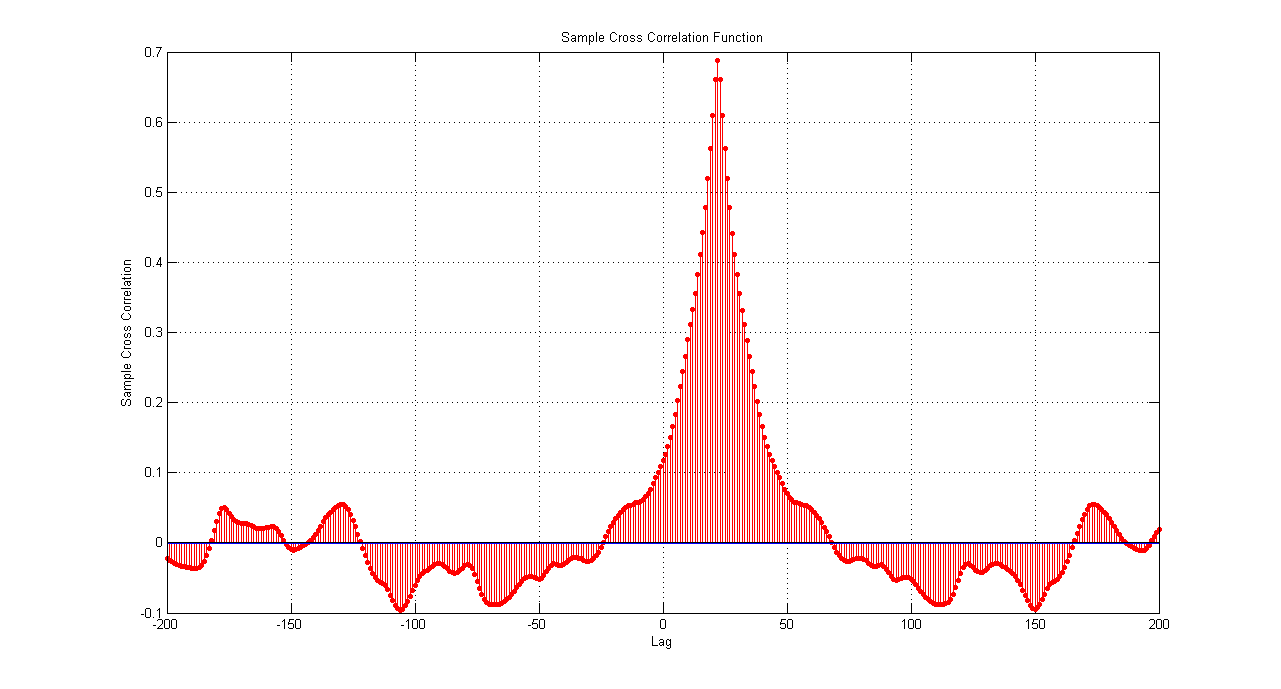
\includegraphics[width=\textwidth]{./img/crosscorr.png}
	\caption{An example cross-correlation between two signals, generated through Matlab modelling}
	\label{fig:crosscorr}
\end{figure}

\noindent
In its current state, the algorithm is functional both when modelled in Matlab, and on the DSP, however it is not suitably up to speed and takes far too long to process the data.
This can be improved by using features of how the data is stored and how the calculations are achieved.
Many of the loops over the data can be removed and replaced by a couple of simple functions, drastically reducing the time taken.
